\chapter{Statische Trajektorienoptimierung} \label{chap:statische_Optimierung}
% Heuristik bei der Trajektorienpalnung erwähnen (Klasse der Optimalen Trajektorie einfach vorgeben)
% Direkte Optimierungsverfahren: Simplex
% Indirekte OV: ...
% Beispiel Lenkruck: Optimierung
% Ziel bremsung als Planung ohne Freiheit grade mit singularität beschreiben.
% Auch zur Identifikation geeignet! Beispiel Reifenkennlinie
% parametrischer Trajektorienplanung

\section{Statische Optimierung}
\begin{figure}[h]
\psfrag{b}[cr][cr][1.0]{$x_2$}
\psfrag{a}[cr][cr][1.0]{$x_1$}
\psfrag{j}[cc][cc][1.0]{$J(x)=\text{const.}$}
\psfrag{o}[cr][cr][1.0]{$x^\ast$}
\psfrag{h}[cr][cr][1.0]{$h(x)=0$}
\psfrag{g}[cl][cl][1.0]{$g(x) = 0$}
	\centering
  	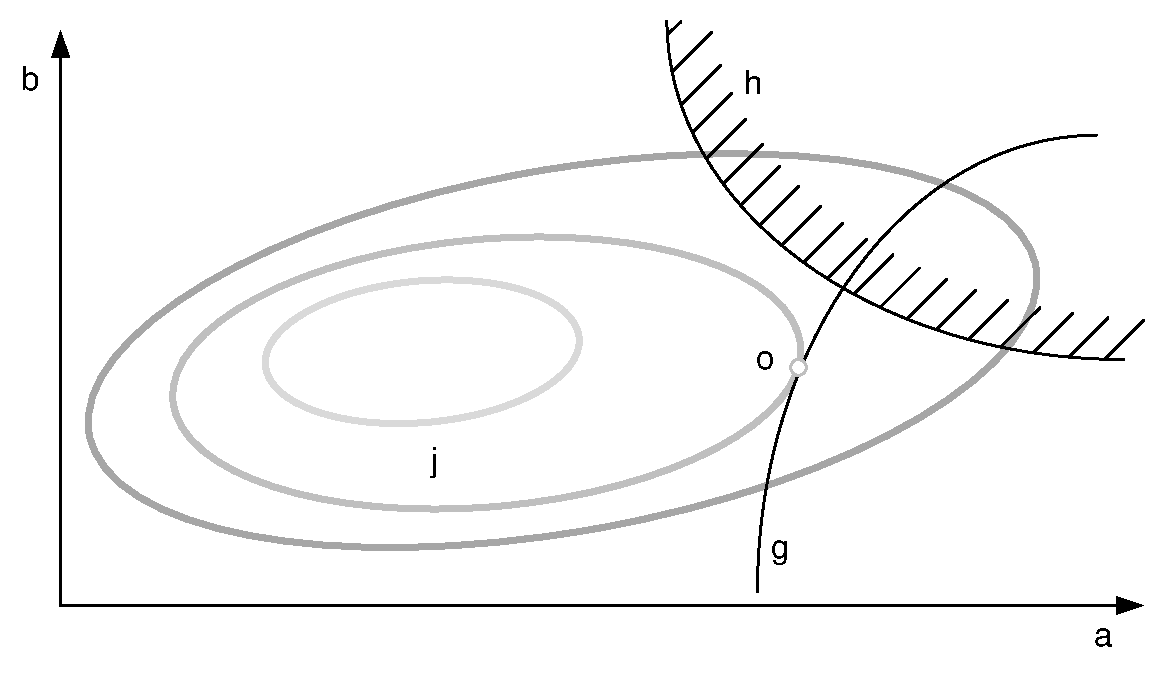
\includegraphics[width=.7\textwidth,clip, trim = 0cm 0cm 0cm 0cm]{2_Darstellung_statische_Optimierung.eps}
		\vspace{-0.1cm}
  	\caption{todo}
    \label{fig:grundidee_nmpc}
		\vspace{-0.2cm}
\end{figure} 
\begin{align}
	\min_{x\in \mathbb R^n} \quad & f(x) &\text{(Kostenfunktion)}
\end{align}

Hinreichende Bedinung für lokales Minimum: % Graichen Skript Satz 3.2
\begin{align}
	\nabla f(x^\ast) &= 0 \\
	\nabla^2 f(x^\ast) &> 0 \quad (\text{positiv definit})
\end{align}

... und unter Berücksichtigung von Nebenbedingungen
\begin{align}
	\min_{x\in \mathbb R^n} \quad & f(x) & & & &\text{(Kostenfunktion)}\\
	\text{u.d.N.} 	 \quad &g_i(x) = 0, & i &= 1, \ldots, p \quad & &\text{(Gleichungsbeschränkungen)} \\
						& h_i(x) \leq 0,  & i &= 1, \ldots, q & &\text{(Ungleichungsbeschränkungen)}
\end{align}

Lagrange-Funktion
\begin{align}
	L(x,\lambda,\mu) = f(x) + \sum_{i=1}^p \lambda_i g_i(x) + \sum_{i=1}^q\mu_i h_i(x)
\end{align}
mit Lagrange-Multiplikatoren $\lambda = [\lambda_1, \ldots, \lambda_p]^\T$ und $\mu = [\mu_1, \ldots, \mu_q]^\T$

		\subsection{Karush-Kuhn-Tucker-Bedingungen}
		Notwendige Optimalitätsbedingung 1. Ordnung % Graichenskipt Satz 4.1
\begin{align}
	\nabla_x L(x^\ast,\lambda^\ast,\mu^\ast) &= 0 \\
	g_i(x^\ast) &= 0, & i&=1,\ldots, p \\
	h_i(x^\ast) &\leq 0, & i&=1,\ldots, q \\
	\mu_i^\ast &\geq 0, & i&=1,\ldots, q \\
	\mu_i^\ast h_i(x^\ast) &= 0, & i&=1,\ldots, q
\end{align}		

	\section{Optimierung von Trajektrienscharen} 
	% Sigmoid, Polynome etc.
	% Parametriertes Einparken
	\section{Elastische Bänder und Potentialfelder} % Vergleich mit NMPC
	
	\cite{koren1991potential} % Inherentes Problem.
	\section{Bewertung}